This option allows users to generate synthetic ground motions for a
target seismic event. In order to do so, the stochastic ground motion
model is selected from the drop-down menu, as shown
in \Cref{fig:stochastic_loading}. Depending on the model selected, the
user will be asked to enter the parameters describing the seismic
event that the synthetic motion should emulate. In the current
release, users can only select the model derived by Vlachos et
al. (2018) \cite{vlachos2018predictive}. Additionally, users can
provide a seed for the stochastic motion generation if they desire the
same suite of synthetic motions to be generated on multiple occasions.
If the seed is not specified, a different realization of the time history
will be generated for each run based on the input parameters. The backend
application that generates the stochastic ground motions relies
on \texttt{smelt}, a modular and extensible C++ library for generating
stochastic time histories. Users interested in learning more about the
implementation and design of
\texttt{smelt} are referred to its
\href{https://github.com/NHERI-SimCenter/smelt}{GitHub repository}.

All input parameters can be specified as random variables by entering
a string in the parameter field. Please note that information for the
inputs that are identified as random variables needs to be provided in
the \texttt{UQ} tab.

\begin{figure}[!htbp]
  \centering {
    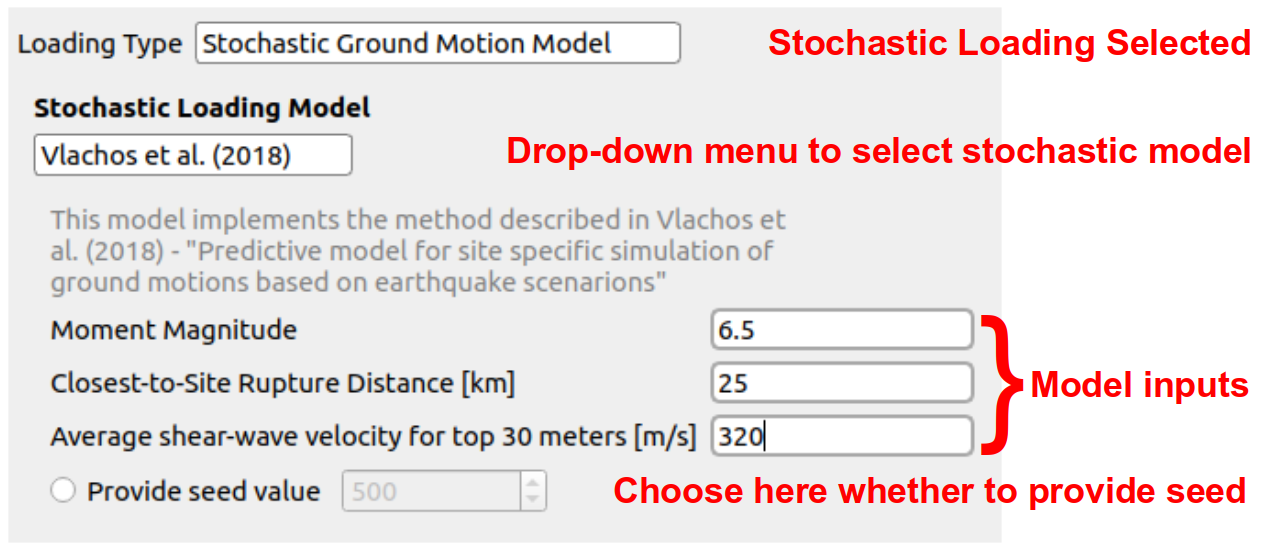
\includegraphics[width=0.8\textwidth]
    {usage/figures/stochastic_loading.png} }
  \caption{Stochastic Ground Motion Event}
  \label{fig:stochastic_loading}
\end{figure}
